\documentclass[../main.tex]{subfiles}
% 2.1.1 Was ist es?
Der Begriff der Interferenz beschreibt das Verhalten von Wellen bei Überlagerungen.

% 2.1.2 Grundsatz
Grundsätzlich heißt es in der Physik, dass bei der Überlagerung von Wellen ihre Amplituden addiert werden \cite{interferenz_grundsatz}. Das heißt, dass z.B. das Aufeinanderstoßen zwei gleich hoher Wellen zu einer verdoppelung der Amplitude führt (Abb. \ref{fig:interferenz-konstruktiv}).

\begin{figure}[ht]
    \centering
    \begin{subfigure}[b]{0.35\textwidth}
        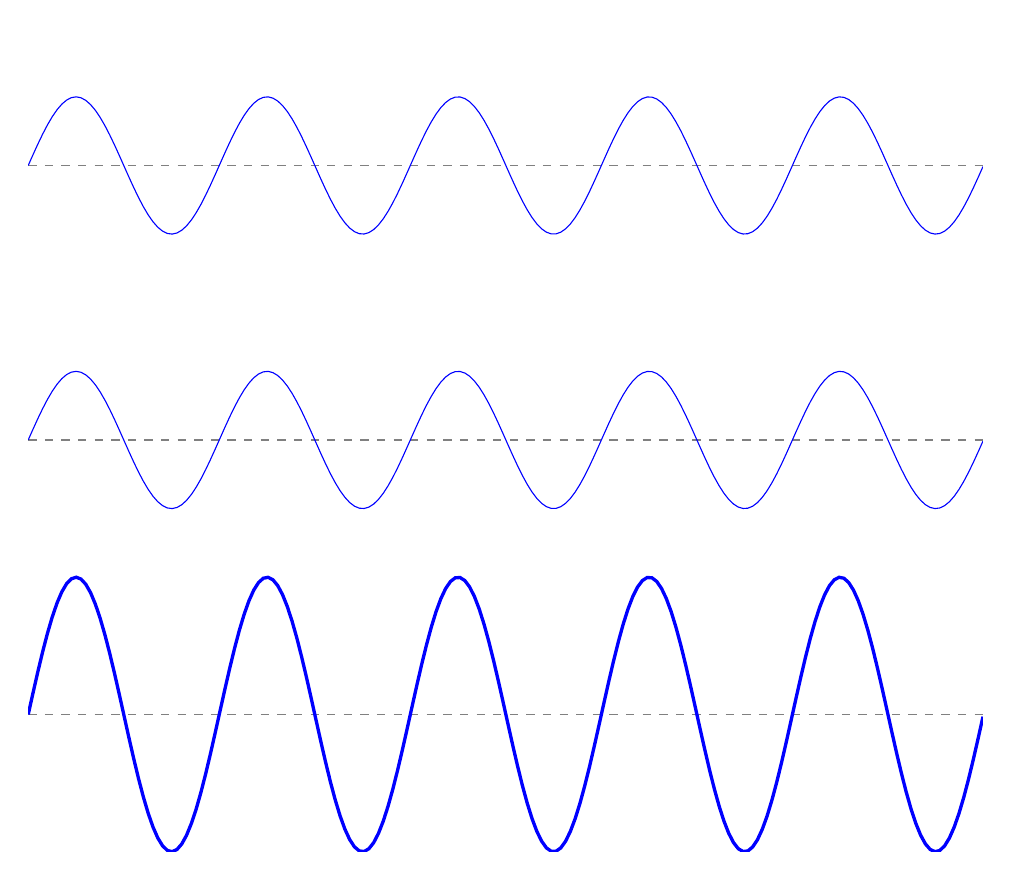
\begin{tikzpicture}
        \begin{axis}[
            xmin=0,xmax=31.4,
            ymin=-3,ymax=3,
            ticks=none,
            axis line style=white,
            scale only axis,
            domain=0:31.4,
            width=\textwidth,
        ]
            \addplot[gray,dashed,thin]{2};
            \addplot[samples=200,blue] {sin(deg(x))/2+2};
            \addplot[gray,dashed,thin]{0};
            \addplot[samples=200,blue] {sin(deg(x))/2};
            \addplot[gray,dashed,thin]{-2};
            \addplot[samples=200,blue,very thick] {sin(deg(x))-2};
        \end{axis}
        \end{tikzpicture}
        \caption{Konstruktive Interferenz}
        \label{fig:interferenz-konstruktiv}
    \end{subfigure}
    \hspace{0.5cm}
    \begin{subfigure}[b]{0.35\textwidth}
        \begin{tikzpicture}
        \begin{axis}[
            xmin=0,xmax=31.4,
            ymin=-3,ymax=3,
            ticks=none,
            axis line style=white,
            scale only axis,
            domain=0:31.4,
            width=\textwidth,
        ]
            \addplot[gray,dashed,thin]{2};
            \addplot[samples=200,blue] {sin(deg(x+3.14))/2+2};
            \addplot[gray,dashed,thin]{0};
            \addplot[samples=200,blue] {sin(deg(x))/2};
            \addplot[gray,dashed,thin]{-2};
            \addplot[samples=200,blue,very thick] {-2};
        \end{axis}
        \end{tikzpicture}
        \caption{Destruktive Interferenz}
        \label{fig:interferenz-destruktiv}
    \end{subfigure}
    \caption{Darstellung der Interferenz von zwei Wellen (oben) mit resultierender Welle (unten)}
    \label{fig:interferenz}
\end{figure}

% 2.1.3 Konstruktiv
Man spricht hier also von Konstruktiver Interferenz - wenn zwei Wellen aufeinander treffen, bei denen die Hoch- bzw. Tiefpunkte überlagern. Voraussetzung ist, dass der Gangunterschied zwei koharänter Wellen das Vielfache ihrer Wellenlänge $\lambda$ beträgt.
\begin{equation}
    \label{eq:konstruktive_interferenz}
    \Delta s = m \cdot \lambda
\end{equation}
Das heißt, dass Wellenhochpunkt auf Wellenhochpunkt und Wellentiefpunkt auf Wellentiefpunkt treffen. Daraus folgt, dass die summierte resultierende Welle eine höhere Amplitude hat (Abb. \ref{fig:interferenz-konstruktiv}).

% 2.1.4 Destruktiv
Im Gegenzug heißt destruktive Interferenz, dass ein Wellenhochpunkt auf einen Tiefpunkt zukommt, und eine Welle mit kleinerer Amplitude herauskommt. Dabei kann es auch zur kompletten Auslöschung der Welle kommen. Vorraussetzung ist, dass der Gangunterschied $\Delta s$ ein Vielfaches der Wellenlänge $\lambda$ ist und um $\frac{\lambda}{2}$ verschoben ist.
\begin{equation}
    \label{eq:destruktive_interferenz}
    \Delta s = (m - \frac{1}{2}) \cdot \lambda
\end{equation}
Somit treffen Hochpunkte auf Tiefpunkte und umgekehrt (Abb. \ref{fig:interferenz}).

% 2.1.5 Mathematische Darstellung
Die Ausbreitung der Welle wird als mathematische Formel normalerweise als $f(x, t)$ beschrieben, wo $x$ die Position der Welle und $t$ der Zeitpunkt der Ausbreitung ist. Somit kann die Überlagerung mehrerer Wellen $f_i(x, t)$ am Punkt $x_0$ beim Zeitpunkt $t$ als Summe der einzelnen Wellen betrachtet werden \cite{interferenz_grundsatz}.
\[
    f_{ges}(x_0, t) = \sum_{i}f_i(x_0, t)
\]
% 2.1.6 Warum Grundlage?
Interferenz ist bei der IR-Spektroskopie ein relevanter Begriff, weil das Infrarotlicht nach dem durchdringen einer Substanz am Detektor durch die Interferenz der IR-Wellen ein bestimmtes Wellenmuster aufweist, welches am Detektor ausgemessen und zum Spektrum ausgewertet werden kann. 